\newpage\section{RESULTS}\label{sec3}%Results
%% topic 1 spectral measures (behavioral relevance and physiological distribution on free ears)
%figure box A - F: Free Ears: VSI across bands, VSI LR and VSI RMSE 
\begin{wrapfigure}[31]{r}{9.5cm}
\captionsetup{width=9cm}
\centering
    \raisebox{0pt}[\dimexpr\height-1.4\baselineskip\relax]{
        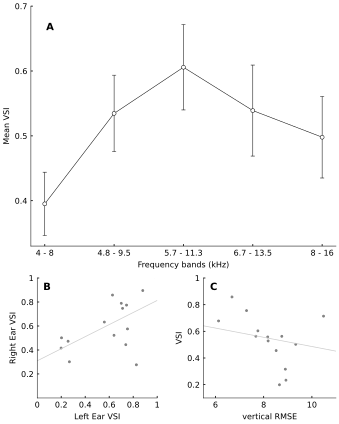
\includegraphics[width=9cm]{../Results/figures/fig2/fig2}}
	\caption{Free ears VSI and localization performance. \textbf{A}, Variation of VSI across five octave bands between 4 and 16kHz. VSI was averaged across sets of DTFs obtained from participants' left and right ears without earmolds. VSI varies significantly and is highest in the 5.7–11.3 kHz band.  \textbf{B}, Left and right ear VSI of each participant in the 5.7-11.3 kHz band. VSIs of the left and right ears were similar. \textbf{C}, Relation between VSI in the 5.7 – 13.5 kHz band and vertical localization accuracy.}
	\label{fig:ef_vsi}
\end{wrapfigure}

\noindent\vspace{-3\baselineskip}
\subsection{Relation between VSI and localization performance free ears}
Participants' directional transfer functions (DTFs) were recorded across the vertical midline with and without earmolds. DTFs from the left and right ear of one participant are shown in \cref{fig:ef_l_r}. To quantify spectral information available for vertical sound localization in the individual sets of DTFs, VSI \citep{trapeau_fast_2016} and spectral strength \citep{middlebrooks_individual_1999} were computed in 5 octave bands between 4 and 16 kHz (4–8 kHz, 4.8–9.5 kHz, 5.7–11.3 kHz, 6.7–13.5kHz, 8–16kHz). Spectral information of participants’ free ears varied among frequency bands (Kruskal-Wallis test, VSI: $p = 0.0087$, spectral strength: $p = 10^{-7}$). The dissimilarity between DTFs across elevations (VSI) peaked in the 5.7 – 11.3 kHz band as previously reported by \citet{trapeau_fast_2016} (\cref{fig:ef_vsi} A). The VSIs of all participants in this band are shown in \cref{fig:ef_vsi} B. Participants' left and right ears had similar VSI (Spearman correlation between the VSI of left and right ears in the 5.7 – 11.3 kHz band: R = 0.45, $p = 0.0897$). Spectral strength, i.e., the variance within individual DTFs, indicated the highest spectral detail in the neighboring 6.7-13.5 kHz band. When joining these two bands for the analysis, VSI correlated with vertical localization accuracy (\cref{fig:ef_vsi} C) and vertical SD (free ears VSI in the 5.7 - 13.5 kHz band compared to vertical localization: RMSE: R = -0.58, $p = 0.0249$, EG: R = 0.15, $p = 0.6025$, SD: R = -0.58, $p = 0.0249$). No correlation was found between behavioral metrics and VSI in the other frequency bands. Spectral strength did not correlate with behavior in the tested frequency bands.

%\newpage
%% topic 2 spectral effect of molds (spectral impact of molds, physiological plausibility, distribution across participants, m1m2 spectral compare)
\subsection{Earmolds reduced spectral information in the 5.7-11.3 kHz band}

Application of silicone molds to the Pinnae altered spectral cues in the 4-16 kHz band. Both sets of earmolds attenuated the prominent spectral notch and the neighbouring spectral peak situated in the 5-12 kHz band (\cref{fig:spectral_change}, A-C). Similar effects have been observed in previous studies using molds to modify spectral cues (\citet{trapeau_fast_2016}, \citet{wanrooij_relearning_2005}, \citet{hofman_relearning_1998}). Comparing VSIs of participants' modified and free ears in the 5.7-11.3 kHz band showed that earmolds reduced the amount of spectral information available for elevation discrimination (\cref{fig:molds_vsi} B, differences between VSI of free and modified ears; Free ears: 0.61 $\pm$ 0.04, vs Molds 1: 0.45 $\pm$ 0.05, $p = 0.0022$, vs molds 2: 0.39 $\pm$ 0.04, $p = 0.0036$). Both sets of earmolds led to similar levels of VSI reduction compared to participants' free ears (free ears VSI reduction caused by molds 1: 0.18 $\pm$ 0.06 vs molds 2: 0.18 $\pm$ 0.06, $p = 0.1973$).The relation between VSIs of participants' left and right ears persisted after mold insertion but was not significant for the second set of earmolds (molds 1: R = 0.56, $p = 0.0336$, molds 2: R = 0.53, $p = 0.064$). \cref{fig:molds_vsi} A shows the VSI of all participants with modified and free ears.

\subsection{Acoustic changes occurred at similar frequencies across participants and were different for both sets of earmolds}

To confirm whether spectral changes occurred at similar frequencies across participants but at different frequencies between both sets of molds, the probability of spectral change induced by the earmolds was mapped for each frequency bin and elevation (\cref{fig:spectral_change} D-F). Spectral changes were defined as the absolute differences between DTFs measured before and after mold insertion above a given threshold. This threshold was a participant-specific measure of spectral difference across DTFs with free ears and was defined by the mean RMS difference across all combinations of DTFs (in dB) at each elevation (average across participants: 4.89 dB $\pm$ 0.15). Based on these thresholds, binary maps of spectral changes were created for each set of earmolds and participant (above-threshold changes were set to 1, all other values were set to 0). The average of these maps across participants shows the proportion of participants for which earmolds induced spectral changes above the threshold at each frequency bin and elevation.

%figure box A - F: DTFs of free vs modified ears and spectral change p
\begin{figure}[h]
\centering
	\centerline{\includegraphics[width=15cm, center]{../Results/figures/fig3/fig3}}
	\caption{Acoustic effect of the earmolds. \textbf{A}, Mean across participants' DTFs with free ears. \textbf{B-C}, Mean across participants' DTFs with modified ears. \textbf{D-E}, Probability maps showing the proportion of participants for which the molds induced marked changes in spectral amplitude at each elevation and frequency bin. \textbf{F}, Probability map showing the proportion of marked changes between the first and second set of molds.}
        \label{fig:spectral_change}
\end{figure}

% Figure box VSI and VSI dissimilarities across conditions
\begin{figure}[t]
\floatbox[{\capbeside\thisfloatsetup{capbesideposition={right,top},capbesidewidth=8cm}}]{figure}[\FBwidth]
{\caption{VSI and VSI dissimilarity across pinna shapes. \textbf{A}, Left and right ear VSI in the 5.7–11.3 kHz band. Each dot represents one participant. Grey dots show VSI values of free ears, blue and red dots represent VSI values with earmolds 1 and 2, respectively. Relations between left and right ear VSI are shown by regression lines. The similarity between left and right ear VSI persisted after mold insertion. \textbf{B}, VSI with and without molds in the 5.7–11.3 kHz band. Both sets of molds reduced VSI significantly. \textbf{C}, VSI dissimilarities across participants in the 5.7-13.5 kHz band. Grey dots show the VSI dissimilarity of free left and right ears between all combinations of two participants. Each colored dot shows the VSI dissimilarity between pinna shapes of one participant. Blue and red dots indicate dissimilarity between free ears and the first and second set of molds, respectively. Yellow dots indicate VSI dissimilarity between both sets of earmolds. The outline of the grey dot cloud largely includes the colored dots, indicating that acoustic differences induced by the molds did not exceed acoustic differences between participants' natural ears. \textbf{D}, VSI dissimilarities between the three pinna shapes in the 5.7-13.5 kHz band. VSI dissimilarity between free ears and the first earmolds was similar to VSI dissimilarity between the first and second set of molds.}
\label{fig:molds_vsi}}
{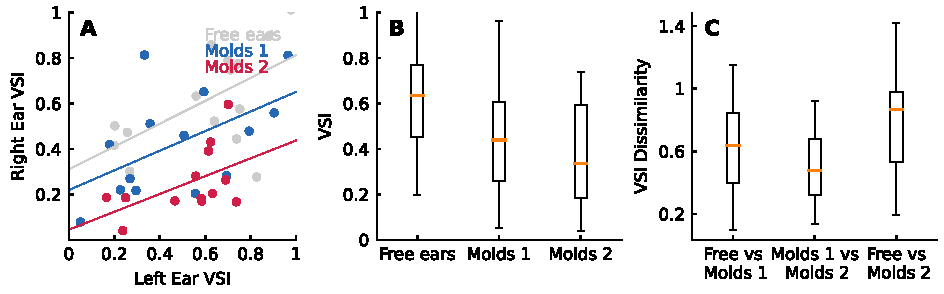
\includegraphics[width=10cm]{../Results/figures/fig4/fig4}}
\end{figure}

\subsection{Consecutive DTFs were equally dissimilar and physiologically plausible}

Each pair of earmolds modified the previously adapted set of DTFs. To test whether spectral differences that were consecutively induced by the molds were in the same range, VSI dissimilarities between the three different pinna shapes (ears free, earmolds 1 and earmolds 2) were computed in the 5.7–13.5 kHz frequency band. The dissimilarity between participants' free ears and the first set of earmolds was comparable to the dissimilarity between the first and the second set of molds (\cref{fig:molds_vsi} D, VSI dissimilarity in the 5.7–13.5 kHz band, free ears and molds 1:  0.64 $\pm$ 0.06 vs molds 1 and molds 2:  0.51 $\pm$ 0.05: $p = 0.2544$). The second set of earmolds induced larger spectral differences to participants' free ears than the first set (VSI dissimilarity free ears and molds 1:  0.64 $\pm$ 0.06 vs free ears and molds 2: 0.8 $\pm$ 0.06; $p = 0.0005$).%\subsection{Acoustic differences caused by the molds were within the physiological range}
To confirm that spectral changes induced by the earmolds were physiologically plausible, VSI dissimilarities between free and modified ears of each participant were compared to VSI dissimilarities between all possible pairs of participants’ free ears (\cref{fig:molds_vsi} C). The overlap of distributions shows that spectral changes induced by both sets of molds were comparable in magnitude to the natural spectrum of differences between individuals’ ears.

%% topic 3 behavior (mold impact on behavior, acoustic explanation)
\subsection{Earmolds reduced vertical localization performance}

Insertion of earmolds degraded vertical localization performance (see \cref{fig:adaptation}, days 0 and 5; one-tailed Wilcoxon signed rank test of vertical localization performance; ears free vs molds 1; RMSE: $p = 3  \times 10^{-5}$, EG: $p = 3 \times 10^{-5}$, SD: $p = 0.0062$, ears free vs molds 2; RMSE: $p = 0.0005$, EG: $p = 0.0005$, SD: $p = 0.0005$). On the horizontal plane, only the standard deviation of responses increased (one-tailed Wilcoxon signed rank test of horizontal localization performance; ears free vs molds 1; SD: $p = 0.04$, ears free vs molds 2: SD: $p = 0.005$). Both sets of earmolds caused a similar decrease of vertical localization performance (mold induced drop in vertical localization performance, two-tailed Wilcoxon signed rank test; molds 1 vs molds 2 ; EG: $p = 0.465$, RMSE: $p = 0.700$, SD: $p = 0.123$).

% Learning plot
 \begin{figure}[ht]
	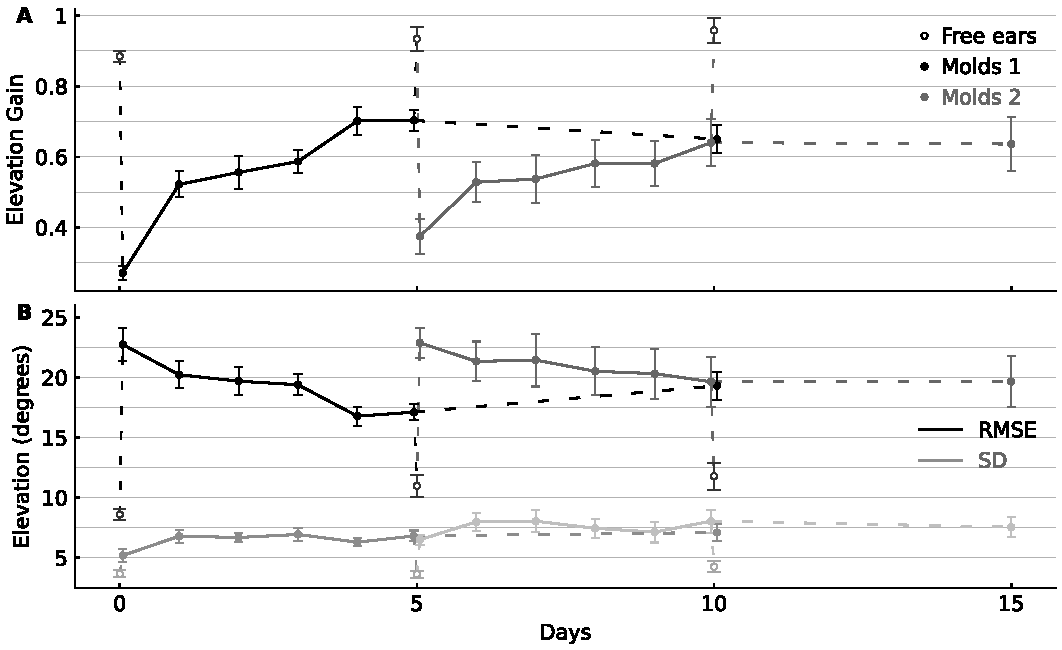
\includegraphics[width=18cm, center]{../Results/figures/fig5/fig5}
	\caption{Time course of vertical localization performance. White dots indicate performance with free ears, black and grey dots indicate performance with molds 1 and molds 2, respectively. Data points represent the mean across participants (ears free: n = 15, molds 1: n = 14, molds 2: n = 13). Errorbars show the standard error. Slim dotted lines plot changes in localization performance after mold insertion and removal. Thick dotted lines show differences between the last test of the adaptation period and the final test of adaptation persistence with each earmold. \textbf{A}, Evolution of EG throughout the two consecutive adaptation periods. Participants EG was reduced by both sets of earmolds and recovered significantly within 5 days of adaptation. No differences in adaptation rate and persistence were found between the first and second set of earmolds. \textbf{B}, placeholder placeholder placeholder placeholder placeholder placeholder placeholder placeholder placeholder placeholder placeholder placeholder placeholder placeholder placeholder placeholder placeholder placeholder placeholder placeholder placeholder placeholder placeholder placeholder placeholder placeholder placeholder placeholder placeholder placeholder placeholder placeholder placeholder placeholder placeholder placeholder placeholder placeholder placeholder placeholder placeholder placeholder placeholder placeholder placeholder placeholder placeholder placeholder placeholder }
        \label{fig:adaptation}
\end{figure}

\subsection{Effects of VSI dissimilarity between pinna shapes on localization accuracy}

To investigate whether acoustic and behavioral effects of the earmolds were related, the VSI dissimilarity between DTFs in the 5.7 – 13.5 kHz band with and without molds was compared to the decrease in participant’s localization performance after insertion of the earmolds. A trend of increasing vertical RMSE for larger acoustic differences was found for the first set of earmolds (\cref{fig:vsi_dis_rmse} A, Spearman correlation of VSI dissimilarity between free ears and molds 1 and increase in vertical RMSE after mold 1 insertion: R = 0.43, $p = 0.122$). No such trend was found for vertical localization and VSI dissimilarity between free ears and the second set of molds (\cref{fig:vsi_dis_rmse} B, Spearman correlation of vertical RMSE in the first test with molds compared to free ears baseline and VSI dissimilarity: R = - 0.18, $p = 0.5926$). Because initial vertical localization accuracy with the second earmolds could additionally depend on acoustic similarities to the previously learned set, differences in localization performance between the final test with earmolds 1 and the initial test with the earmolds 2 were compared to the VSI dissimilarity between both sets of molds. A trend of increasing vertical error with greater acoustic dissimilarity between the first and second set of earmolds was found (\cref{fig:vsi_dis_rmse} C, Spearman correlation of increase in vertical RMSE from the last test with molds 1 to the first test with molds 2 and VSI dissimilarity between consecutive earmolds: R = 0.35, $p = 0.2847$).

 % VSI dissimilarity and RMSE
 \begin{wrapfigure}[15]{l}{12.5cm}
\centering
    \raisebox{0pt}[\dimexpr\height+2.5\baselineskip\relax]{
        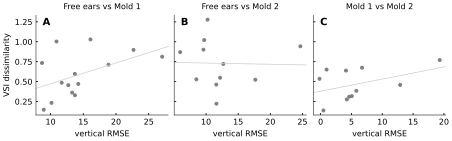
\includegraphics[width=12cm]{../Results/figures/fig6/fig6}}
	\caption{caption title. \textbf{A}, caption}
	\label{fig:vsi_dis_rmse}
\end{wrapfigure}
\noindent%\vspace{-3\baselineskip}

 %% topic 4 adaptation(general adaptation, rate of adaptation m1/m2, generalisability, aftereffect, persistence)
 
 \subsection{Participants consecutively adapted to two novel sets of DTFs}
 
Participants wore two different sets of earmolds during two consecutive 6-day adaptation periods. Adaptation was driven by multisensory experience while wearing the molds throughout the day, accompanied by five sessions of daily sensory-motor training at the lab. Vertical sound localization performance improved significantly for both sets of earmolds except for response variability (SD), which increased throughout the adaptation period (Fig 1, one-tailed Wilcoxon signed rank tests of first vs last day of molds; Earmolds 1: EG: p = 3x10-5, RMSE: p = 6x10-5, SD: p = 0.008; Earmolds 2: EG: p = 3x10-4, RMSE: p = 0.032, SD: p = 0.004). As expected, horizontal localization was not affected by adaptation to the earmolds (Fig 3 B, one-tailed Wilcoxon signed rank tests of first vs last day of molds; Earmolds 1; RMSE: p = 0.555, SD: p = 0.467; Earmolds 2; RMSE: p = 0.485, SD: p = 0.515).

\subsection{No difference between rates of adaptation to first and second earmolds}

To investigate possible effects of metaplasticity (i.e., an effect of the previous adaptation to earmolds 1 on the subsequent adaptation to earmolds 2) the rates of adaptation to the first and second earmolds were compared. To assess the rate of adaptation across participants independent of initial acoustical disruption caused by the earmolds, the increase in vertical localization accuracy during adaptation (performance on day 0 vs day 6) was divided by the initial decrease caused by the molds. Individual adaptation rates varied continuously and did not fall into discernable groups. No difference was found between the two sets of earmolds (two-tailed Wilcoxon signed rank test of Molds 1 vs Molds 2, Reduction of vertical RMSE from day 0 to day 6 divided by initial increase; Earmolds 1: 0.66 +/- 0.06 vs Earmolds 2:  0.74 +/- 0.09, p = 0.413). Individual adaptation performance with the first set of earmolds was positively related to adaptation performance with the second set of molds, although not significant (R = 0.47, p = 0.142). No correlation was found between vertical spectral information of the earmolds in the 3.7 – 12.9 kHz band and adaptation performance.

 \subsection{Adaptation was generalizable}

To rule out the possibility of participants memorizing location-specific spectral features of the training stimuli in the localization test, the test was repeated with a subset of six participants on the last day of each adaptation period using stimuli of random spectral content (USOs). The effect of USO stimuli on vertical localization error did not differ between adapted earmolds and free ears indicating that generalizable perceptual learning had taken place (Friedman test; differences in vertical RMSE between pink noise and USO localization across conditions; Ears free: -0.38 +/- 1.82, Earmolds 1: 2.5 +/- 0.46, Earmolds 2: -0.15 +/- 0.45, p = 0.135).

 \subsection{No aftereffect on free ears localization performance after mold removal}

Previous studies reported the absence of an aftereffect on localization performance with free ears after adaptation to new spectral cues for sound localization (Hofman 1998, Trapeu and Schönwiesner 2015). To confirm these findings, free ears localization accuracy was measured immediately after mold removal at the end of each adaptation period. 
No aftereffect was present for elevation gain but. An increasing impact on participants’ vertical localization accuracy with their native ears was observed after each adaptation period (see Fig. 1 B, one-tailed Wilcoxon signed rank test, vertical RMSE; free ears baseline vs free ears day 5: p = 0.002, free ears baseline vs free ears day 10: p = 6x10-4). 

% response evolution plot
 \begin{figure}[hb]
	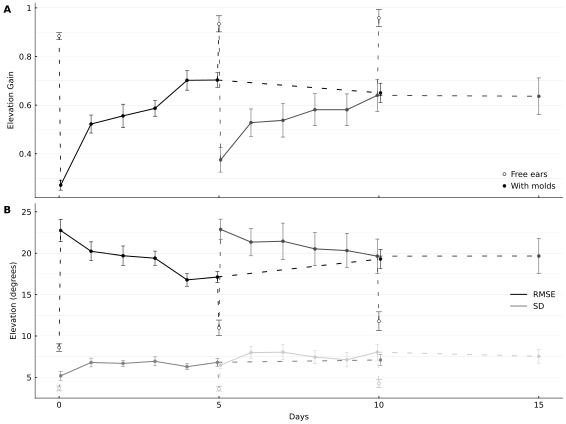
\includegraphics[width=14cm, left]{../Results/figures/fig7/fig7}
	\caption{caption}
        \label{fig:response_evo}
\end{figure}

\subsection{Effects of mold induced acoustic differences on adaptation}
The relation between acoustic differences and behavior was still visible on the last day of the adaptation period (\cref{fig:vsi_dis_rmse} B, Spearman correlation of vertical RMSE in the last test with molds compared to free ears baseline and VSI dissimilarity: R = 0.38, p = 0.185).  